% Block diagram of the proposed soft-core (RISC-V + ChibiOS) architecture on Artix-7.
% Render with "make" in this directory (pdflatex + pdftoppm).
\documentclass[tikz,border=8pt]{standalone}
\usepackage[T1]{fontenc}
\usepackage{lmodern}
\usetikzlibrary{positioning,fit,backgrounds,arrows.meta,calc}

\begin{document}
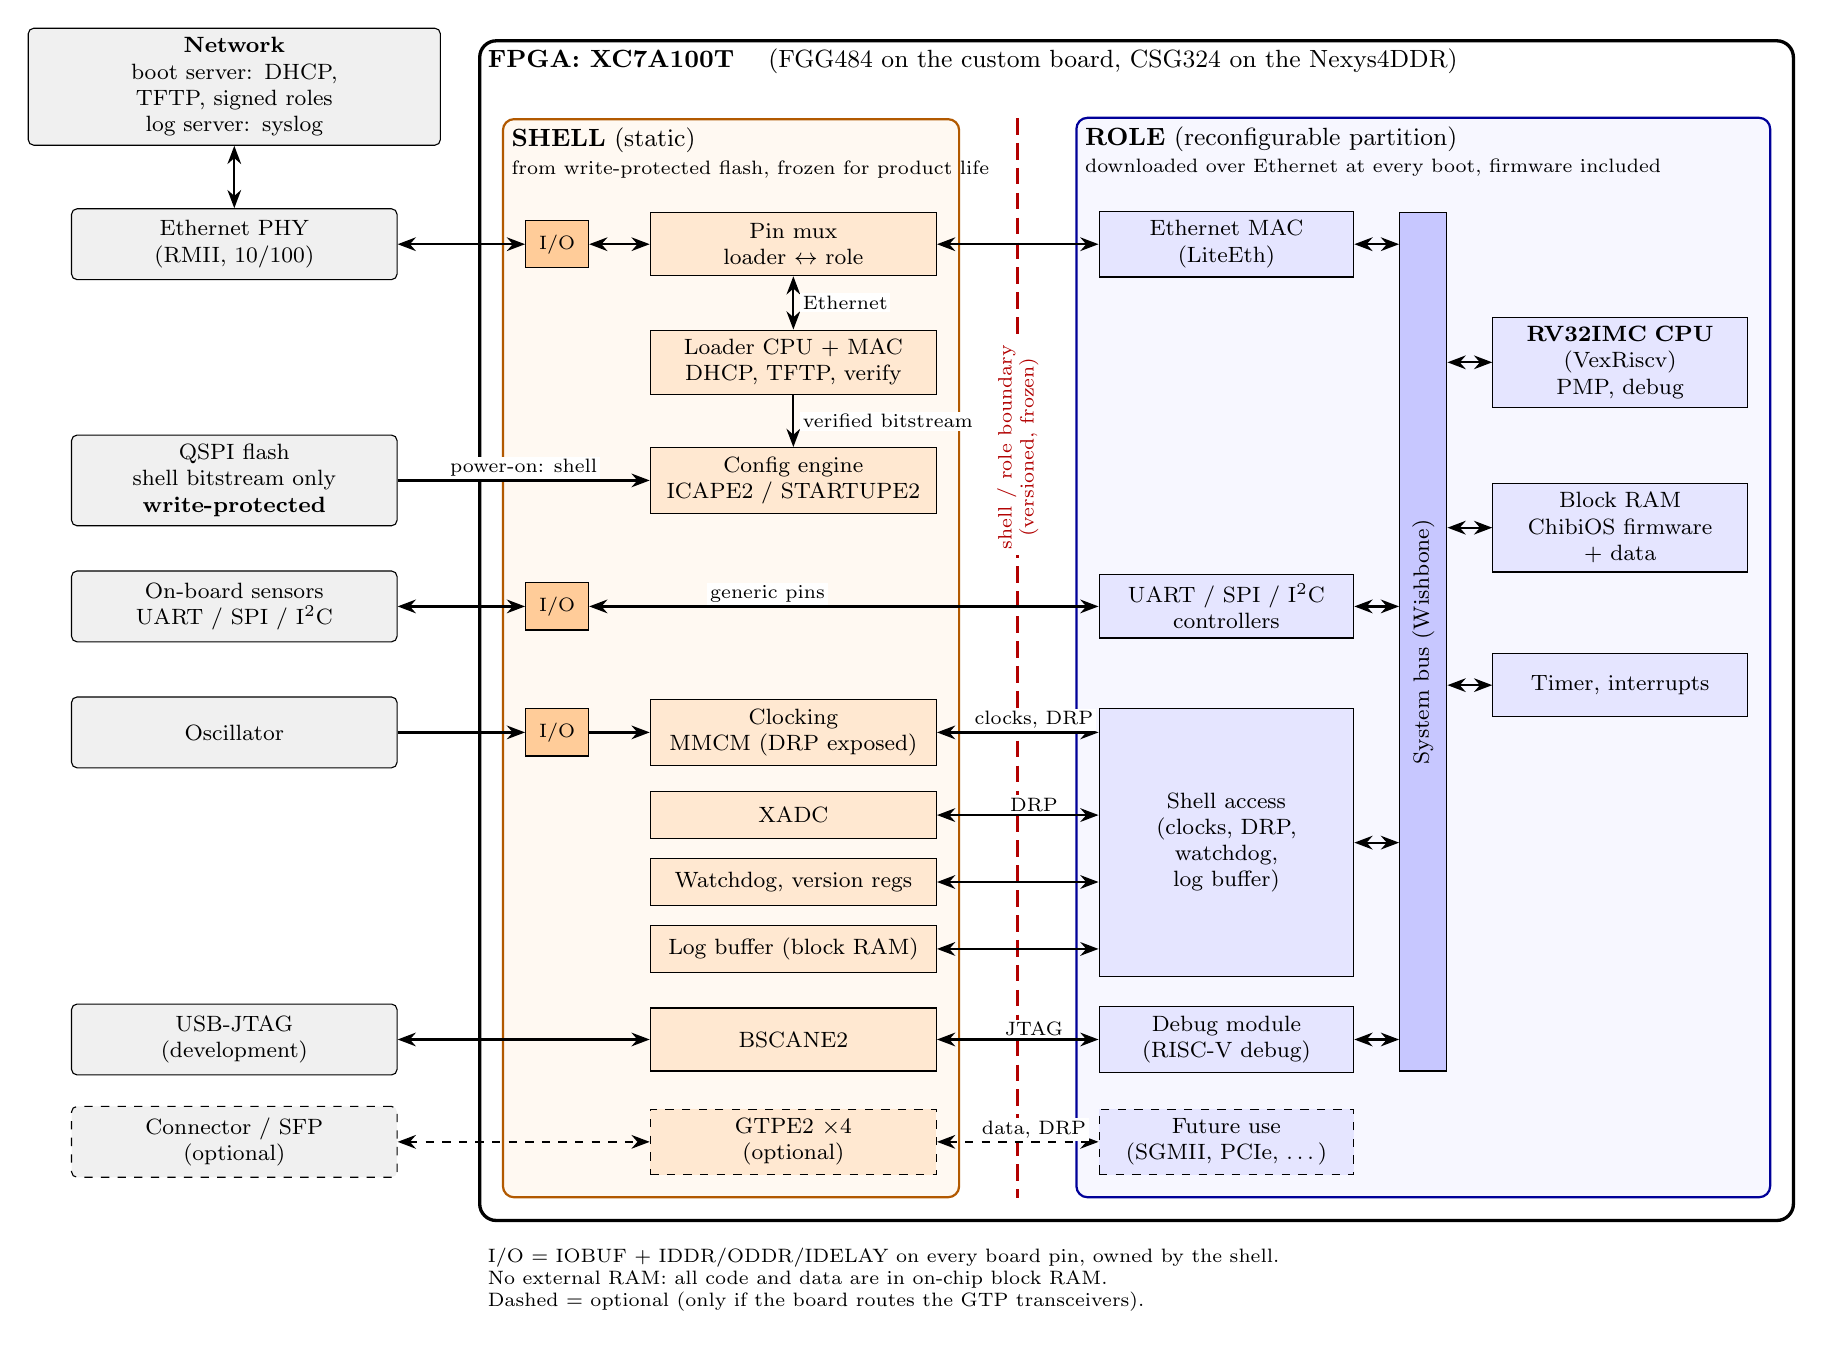
\begin{tikzpicture}[
    >=Stealth,
    font=\footnotesize,
    ext/.style={draw, fill=gray!12, rounded corners=2pt, align=center,
                text width=3.9cm, minimum height=0.9cm},
    shl/.style={draw, fill=orange!18, align=center,
                text width=3.4cm, minimum height=0.8cm},
    rol/.style={draw, fill=blue!10, align=center,
                text width=3.0cm, minimum height=0.8cm},
    io/.style={draw, fill=orange!40, align=center, font=\scriptsize,
               minimum width=0.8cm, minimum height=0.6cm},
    opt/.style={dashed},
    lnk/.style={<->, thick},
    note/.style={font=\scriptsize, fill=white, inner sep=1pt},
  ]

  % Column x positions
  \def\xE{1.0}   % external devices
  \def\xIO{5.1}  % I/O primitives
  \def\xS{8.1}   % shell logic
  \def\xP{13.6}  % role peripherals
  \def\xBus{16.1}% role system bus
  \def\xC{18.6}  % role CPU complex

  % ---------------- External (board) ----------------
  \node[ext, text width=5.0cm] (lan) at (\xE,2.0)
    {\textbf{Network}\\boot server: DHCP, TFTP, signed roles\\log server: syslog};
  \node[ext] (phy)   at (\xE,0)     {Ethernet PHY\\(RMII, 10/100)};
  \node[ext] (flash) at (\xE,-3.0)  {QSPI flash\\shell bitstream only\\\textbf{write-protected}};
  \node[ext] (dev)   at (\xE,-4.6)  {On-board sensors\\UART / SPI / I$^2$C};
  \node[ext] (osc)   at (\xE,-6.2)  {Oscillator};
  \node[ext] (jtag)  at (\xE,-10.1) {USB-JTAG\\(development)};
  \node[ext, opt] (gtpc) at (\xE,-11.4) {Connector / SFP\\(optional)};

  % ---------------- Shell (static) ----------------
  \node[io] (io1) at (\xIO,0)    {I/O};
  \node[io] (io3) at (\xIO,-4.6) {I/O};
  \node[io] (io4) at (\xIO,-6.2) {I/O};

  \node[shl] (mux)   at (\xS,0)     {Pin mux\\loader $\leftrightarrow$ role};
  \node[shl] (ldr)   at (\xS,-1.5)  {Loader CPU + MAC\\DHCP, TFTP, verify};
  \node[shl] (cfg)   at (\xS,-3.0)  {Config engine\\ICAPE2 / STARTUPE2};
  \node[shl] (clk)   at (\xS,-6.2)  {Clocking\\MMCM (DRP exposed)};
  \node[shl, minimum height=0.6cm] (xadc) at (\xS,-7.25) {XADC};
  \node[shl, minimum height=0.6cm] (wdg)  at (\xS,-8.1)  {Watchdog, version regs};
  \node[shl, minimum height=0.6cm] (logb) at (\xS,-8.95) {Log buffer (block RAM)};
  \node[shl] (bscan) at (\xS,-10.1) {BSCANE2};
  \node[shl, opt] (gtp) at (\xS,-11.4) {GTPE2 $\times4$\\(optional)};

  % ---------------- Role (reconfigurable) ----------------
  \node[rol] (eth)  at (\xP,0)     {Ethernet MAC\\(LiteEth)};
  \node[rol] (per)  at (\xP,-4.6)  {UART / SPI / I$^2$C\\controllers};
  \node[rol, minimum height=3.4cm] (csr) at (\xP,-7.6)
    {Shell access\\(clocks, DRP,\\watchdog,\\log buffer)};
  \node[rol] (dbg)  at (\xP,-10.1) {Debug module\\(RISC-V debug)};
  \node[rol, opt] (fut) at (\xP,-11.4) {Future use\\(SGMII, PCIe, \dots)};

  \node[draw, fill=blue!22, minimum width=0.6cm, minimum height=10.9cm]
    (bus) at (\xBus,-5.05) {};
  \node[rotate=90] at (bus.center) {System bus (Wishbone)};

  \node[rol] (cpu)  at (\xC,-1.5) {\textbf{RV32IMC CPU}\\(VexRiscv)\\PMP, debug};
  \node[rol] (ram)  at (\xC,-3.6) {Block RAM\\ChibiOS firmware\\+ data};
  \node[rol] (irq)  at (\xC,-5.6) {Timer, interrupts};

  % ---------------- Links ----------------
  \draw[lnk] (lan) -- (phy);
  \draw[lnk] (phy) -- (io1);
  \draw[lnk] (io1) -- (mux);
  \draw[lnk] (mux) -- (eth);
  \draw[lnk] (ldr) -- node[note, right=2pt] {Ethernet} (mux);
  \draw[->, thick] (ldr) -- node[note, right=2pt] {verified bitstream} (cfg);
  \draw[->, thick] (flash) -- node[note, above] {power-on: shell} (cfg);

  \draw[lnk] (dev) -- (io3);
  \draw[lnk] (io3) -- node[note, pos=0.35, above] {generic pins} (per);
  \draw[->, thick] (osc) -- (io4);
  \draw[->, thick] (io4) -- (clk);
  \draw[lnk] (clk.east) -- node[note, pos=0.6, above] {clocks, DRP} (clk.east -| csr.west);
  \draw[lnk] (xadc.east) -- node[note, pos=0.6, above] {DRP} (xadc.east -| csr.west);
  \draw[lnk] (wdg.east) -- (wdg.east -| csr.west);
  \draw[lnk] (logb.east) -- (logb.east -| csr.west);
  \draw[lnk] (jtag) -- (bscan);
  \draw[lnk] (bscan) -- node[note, pos=0.6, above] {JTAG} (dbg);
  \draw[lnk, opt] (gtpc) -- (gtp);
  \draw[lnk, opt] (gtp) -- node[note, pos=0.6, above] {data, DRP} (fut);

  \foreach \n in {eth, per, csr, dbg}
    \draw[lnk] (\n.east) -- (\n.east -| bus.west);
  \foreach \n in {cpu, ram, irq}
    \draw[lnk] (\n.west) -- (\n.west -| bus.east);

  % ---------------- Regions ----------------
  \begin{scope}[on background layer]
    \node[draw=orange!70!black, fill=orange!5, rounded corners=4pt, thick,
          inner sep=8pt, fit={(io1) (mux) (gtp) (io4) ($(mux.north)+(0,0.9)$)}]
      (shell) {};
    \node[anchor=north west, align=left, font=\small] at (shell.north west)
      {\textbf{SHELL} (static)\\[-1pt]\scriptsize from write-protected flash, frozen for product life};

    \node[draw=blue!60!black, fill=blue!3, rounded corners=4pt, thick,
          inner sep=8pt, fit={(eth) (fut) (cpu) (bus) ($(eth.north)+(0,0.9)$)}]
      (role) {};
    \node[anchor=north west, align=left, font=\small] at (role.north west)
      {\textbf{ROLE} (reconfigurable partition)\\[-1pt]\scriptsize downloaded over Ethernet at every boot, firmware included};

    \node[draw, very thick, rounded corners=6pt, inner sep=8pt,
          fit={(shell) (role) ($(shell.north)+(0,0.7)$)}] (fpga) {};
    \node[anchor=north west, font=\small] at (fpga.north west)
      {\textbf{FPGA: XC7A100T} \quad (FGG484 on the custom board, CSG324 on the Nexys4DDR)};
    \coordinate (bx) at ($(shell.east)!0.5!(role.west)$);
    \draw[red!70!black, very thick, dash pattern=on 6pt off 3pt]
      (bx |- shell.north) -- (bx |- shell.south);
  \end{scope}

  \node[rotate=90, font=\scriptsize, red!70!black, fill=white, inner sep=2pt, align=center]
    at (bx |- cfg.north)
    {shell / role boundary\\(versioned, frozen)};

  % ---------------- Legend ----------------
  \node[anchor=north west, align=left, font=\scriptsize] at ($(fpga.south west)+(0,-0.2)$)
    {I/O = IOBUF + IDDR/ODDR/IDELAY on every board pin, owned by the shell.\\
     No external RAM: all code and data are in on-chip block RAM.\\
     Dashed = optional (only if the board routes the GTP transceivers).};
\end{tikzpicture}
\end{document}
